
\section{Relational abstractors as transformer modules}
\label{sec:abstractors_as_transformer_modules}

In the previous section we considered relational learning
in terms of symbolic message passing operations, where the connection to transformers 
was suggested. In this section, we make the connection more explicit, formulating 
these operations as extensions of transformer architectures.



\subsection{Relational learning using transformers}

In our extended framework, processing occurs in encoder/decoder modules that handle particular types of information,
separated from modules for ``abstract inference.'' The encoders/decoders and the abstractor modules communicate
through cross-attention mechanisms that couple abstract states with specific information in encoder/decoder modules to which they refer in a given problem instance.  The abstract layers are composable to include a hierarchy of abstract modules in which higher order relations are learned from lower level relations, analogous to how convolutional layers are composed in deep neural networks.

The architecture has three types of states: encoder states $E$, decoder states $D$, and abstract states $A$. The encoder states are vectors that represent domain-specific information (e.g., sensory or motor), which are often successfully modeled by standard deep learning frameworks, including standard transformers. The abstract states $A$ are vectors that are learned and processed using similar mechanisms but, critically, without direct exposure to the encoder states $E$.  In particular, the encoder states are separated from the abstract states by a ``relational bottleneck'' that only allows information about relations (that is, inner-products) between encoder states to influence the learning and transformation of abstract states. The Abstractor framework enables domain-specific relations to be modeled in the Encoder, as done by standard transformers, giving the framework more flexibility relative to ESBN. 
%If sensory information is required by the decoder, this can be passed to the decoder states $D$ by standard cross-attention mechanisms of transformers.

\begin{figure}[t]
    \vspace{-3mm}
    \begin{center}
    \begin{tabular}{c}
        \hskip5pt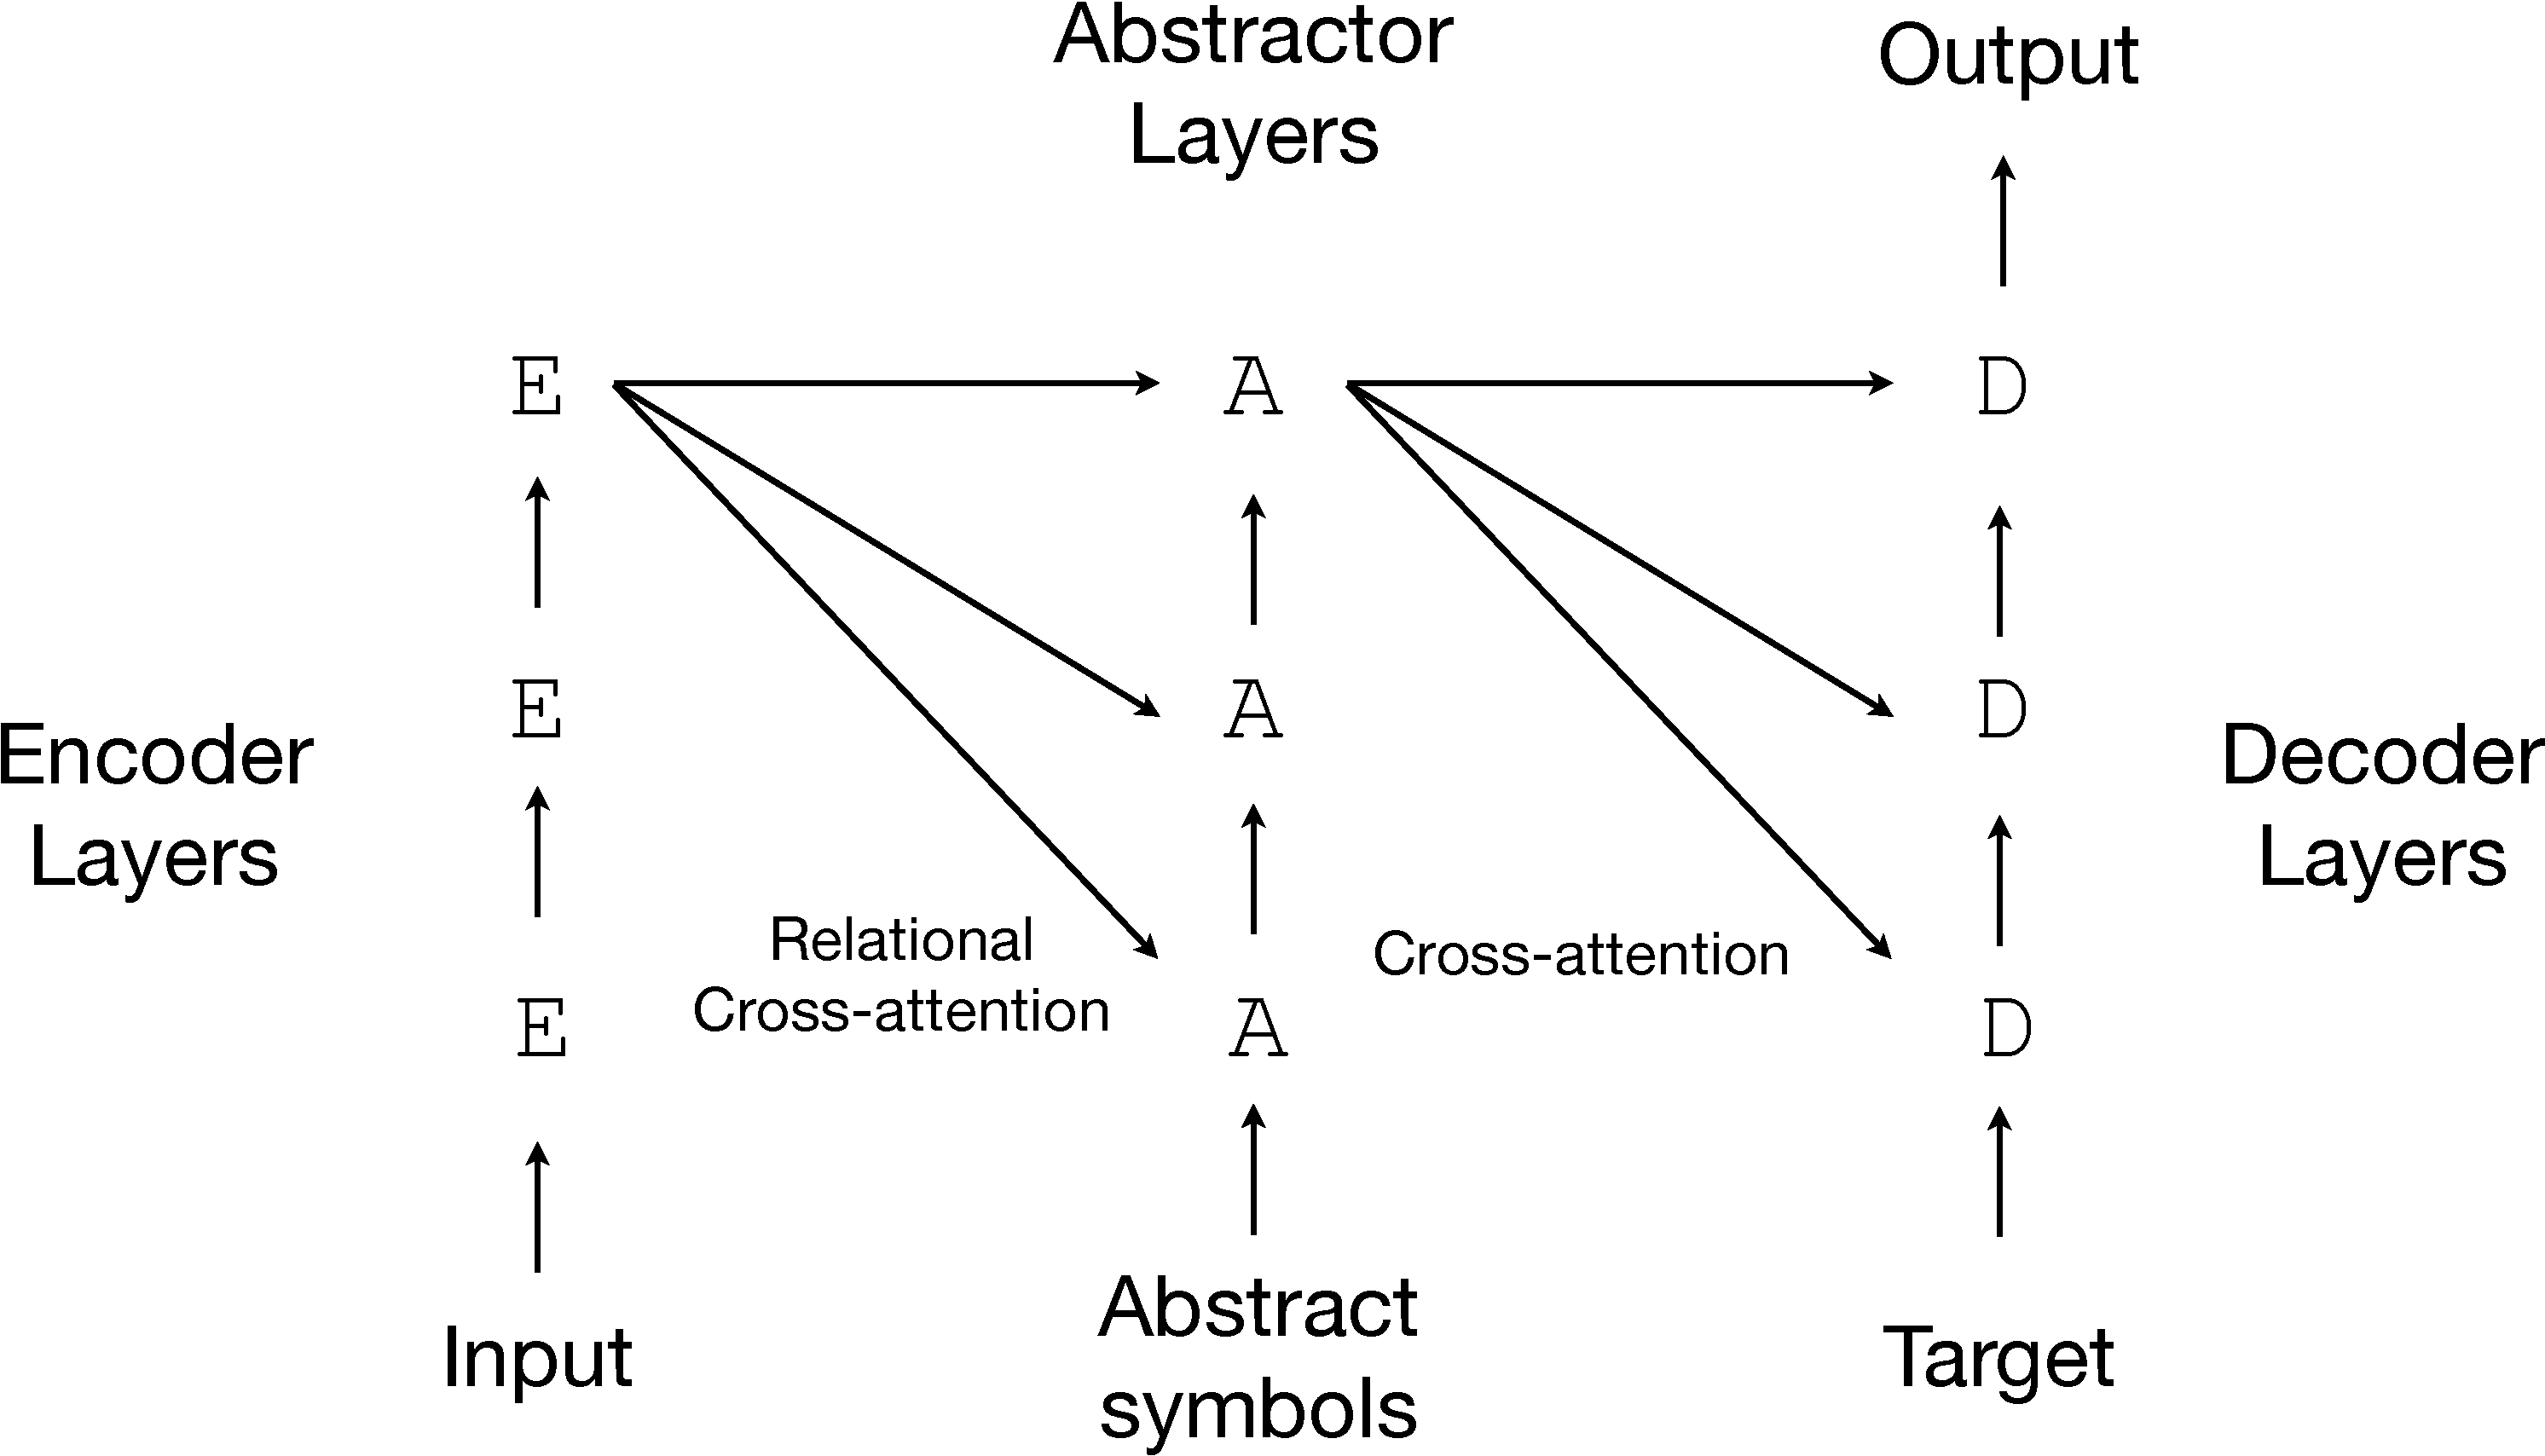
\includegraphics[width=.60\textwidth]{figures/algorithm-diagram3-crop}
    \end{tabular}
    \caption{Algorithmic framework integrating transformers and relational learning, with encoder/decoder layers for
    sensory/motor processes, and abstractor layers for representing relations between encoder and decoder states. For purely relational reasoning the abstract symbols depend only on relations between encoder states, which is a form of the ``relational bottleneck.''}
    \label{fig:algo}
    \vskip-12pt
    \end{center}
\end{figure}



\subsection{Relational cross-attention}

In the message-passing operation \Cref{eq:linear_symbolic_mp}, it is useful to normalize the relations $R$ via a softmax so that they are non-negative and sum to one. Hence, after each symbolic message-passing operation, the updated representation of each symbol involves a convex combination of the other symbols determined by the relations. Suggestively renaming the linear mappings of \eqref{eq:relation_innerproduct} as $W_Q$ and $W_K$, this can be compactly written as
\begin{equation}
    \label{eq:relational_crossattention}
    \begin{split}
        A &= S R, \\
        R &= \Softmax\left((W_K E)^\top (W_Q E)\right) = \Softmax\left(K^\top Q\right),
    \end{split}
\end{equation}
where $S = (s_1, \ldots, s_\m) \in \reals^{d_s \times m}$ is the matrix of symbols and $E
= (o_1, \ldots, o_\m) \in \reals^{d_o \times \m}$ is the matrix of embeddings of input objects. 
The softmax operation is applied column-wise, so that each column sums to one across the rows.
This is essentially the cross-attention operation of transformers, where the queries and keys both come from the input objects, and the values come from the learned input-independent symbols. Hence, we refer to this operation as relational cross-attention and denote it by $\qkv{E}{E}{S}$. 
The $\m\times \m$ matrix $R = (r_{ij})$ is thought of 
as a relation between keys and values, computed in terms of inner products, with column $r_j$ 
encoding the relations between query $q_j$ and the keys $k_1, k_2, \ldots, k_m$. Thus, the transformed 
values are 
\begin{equation*}
    v_j \leftarrow V r_j = \sum_{i=1}^m r_{ij} v_i .
\end{equation*}

In standard transformers, the self-attention operation between encoder 
states is 
\begin{equation*}
    \selfattention{E} \equiv \crossattention{E}{E}{E},
\end{equation*} 
and the cross-attention mechanism between encoder states $E$ and decoder states $D$ takes the form 
\begin{equation*}
     \qkv{D}{E}{E}
\end{equation*}

Given the context of the encoder states $E$, a sequence of abstractor layers transforms the abstract symbols $A = (a_1,\ldots, a_m)$, using two types of attention: $\selfattention{E}$ and 
\textit{relational cross-attention}
\begin{equation*}
    \qkv{E}{E}{A}.
\end{equation*}
The initial abstract state is $S = (s_1,\ldots, s_m)$
with abstract symbols $s_j$ that are task-dependent but input-indendent, trainable using
backpropagation. The relational cross-attention mechanism learns relations among the encoder states and uses those
relations to transform the abstract state. Importantly, the relational cross-attention heads
encode learned relations and attributes, and can be reused across tasks.


Only relational information in the encoder states, computed through inner products,
is used to transform the abstract variables; no information about the encoder states $E$ is directly accessed by the abstract side. For example, an attention head may learn to be directed toward the relevant dimension of an $E$ state (e.g., the color or shape of an object), without being associated with any particular value along that dimension. If the specific representation of $E$ changes, the same abstract relations will hold as long as the transformed inner products are approximately preserved. Thus, an abstractor is constructed to enforce the relational bottleneck 
no matter which transformations are learned by the attention heads.



\subsection{Example}
\label{ssec:set}

We use the game SET to illustrate relational cross-attention.
% JDC: COULD REFERENCE WIKIPEDIA PAGE FOR SET:  https://en.wikipedia.org/wiki/Set_(card_game)
SET is a relatively straightforward but challenging cognitive task that engages reasoning faculties in a deliberative
, attentionally directed manner, requiring several levels of abstraction over sensory embeddings. Players are
presented with 12 cards, each of which contains figures that vary along four dimensions (color, number, pattern, and
shape; see Figure \ref{fig_set}a) and they must find subsets of three cards which obey a deceptively simple rule: along each dimension, all cards in a set must either have the same or unique values (e.g., in Figure \ref{fig_set}, cards with two solid blue/purple diamonds, two striped blue squiggles, and two open blue oblongs: same color, same number, different patterns, different shapes).

Algorithmically, task performance can be described as follows. The visual arrangement of cards is processed into a set of encoder states $E$ by standard deep learning mechanisms. The abstractor, starting in some initial abstract state $A$, transforms the state by the evaluation of attention heads that extract relations between the cards, each head giving a relation between them in a learned attribute.

\def\redcard{\colorbox{red!30}{R}\hskip.2em}
\def\bluecard{\colorbox{blue!30}{B}\hskip.2em}
\def\greencard{\colorbox{green!50}{G}\hskip.2em}
\def\onecard{\fbox{\hskip1pt 1\hskip1pt}\hskip.2em}
\def\twocard{\fbox{\hskip1pt 2\hskip1pt}\hskip.2em}
\def\threecard{\fbox{\hskip1pt 3\hskip1pt}\hskip.2em}

\begin{figure}[t]
\begin{center}
\begin{tabular}{ccc}
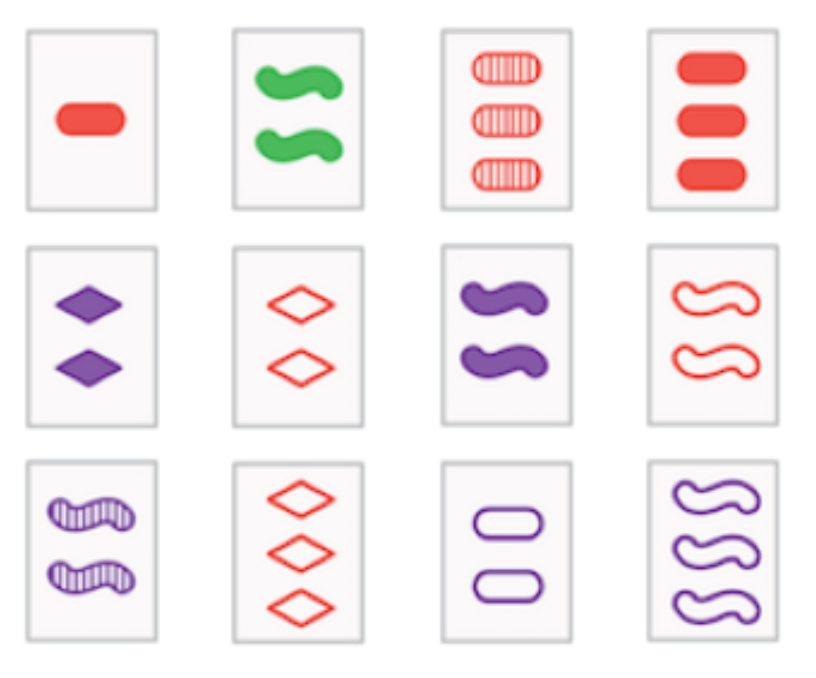
\includegraphics[width=.23\textwidth]{figures/set_example}
& &\\[-1.45in]
&\hskip10pt\ &\renewcommand{\arraystretch}{1.4}
\begin{small}
\begin{tabular}{|c|c|c|}
%\hline
\multicolumn{3}{c}{Attributes of encoder state $E$} \\
\hline
\multicolumn{1}{|c}{\redcard \redcard \redcard} & \multicolumn{1}{|c}{ \redcard\bluecard\greencard} &\multicolumn{1}{|c|}{\redcard\redcard\bluecard} \\
\hline
\hline
%$\frac{1}{3}(s_1+s_2+s_3)$ & $\frac{1}{2}(s_2+s_3)$ & $s_3$ \\
%$\frac{1}{3}(s_1+s_2+s_3)$ & $\frac{1}{2}(s_1+s_3)$ & $s_3$ \\
%$\frac{1}{3}(s_1+s_2+s_3)$ & $\frac{1}{2}(s_1+s_2)$ & $\frac{1}{2}(s_1+s_2)$ \\
$\frac{1}{3}(s_1+s_2+s_3)$ & $s_1$ & $\frac{1}{2}(s_1+s_2)$ \\
$\frac{1}{3}(s_1+s_2+s_3)$ & $s_2$ & $\frac{1}{2}(s_1+s_2)$ \\
$\frac{1}{3}(s_1+s_2+s_3)$ & $s_3$ & $s_3$ \\
\hline
\multicolumn{3}{c}{Transformed abstract symbol $A$}
%\hline
\end{tabular}
\end{small}
%& \\[-1.45in]
%&&\includegraphics[width=.23\textwidth]{ppo-results/epoch_14_decision_boundaries} \vspace{-2mm} \\
\\[10pt]
\scriptsize (a) SET game && \scriptsize (b) Example of symbols/attention
\end{tabular}
\vspace{-1mm}
\end{center}
\caption{Illustration of mechanism used in abstractor layers with relational cross attention using the game of SET (see text for description).
%To provide a basic working of example of abstraction in our framework,
As an example, consider an initial abstract symbol $S = (s_1,s_2,s_3)$ for three cards, and the color attribute.
%, for concreteness.
Suppose a relation is learned such that  $\langle W_Q E_i, W_K E_j\rangle$ is small if cards $i$ and $j$ have different color, and is large if they are the same color.  Then relational cross-attention transforms the initial abstract symbol $S$ as shown in the above table. A multilayer perceptron can learn to discriminate between these three cases. Once learned, the symbol $A$ then can be used to represent abstract ``same/different'' relations for the sequence of inputs.}
\label{fig_set}
\end{figure}


\subsection{Configuring abstractors for different tasks}
\def\module#1{\mbox{\small\texttt{#1}}}

Abstractors can be used to approach a variety of relational learning tasks. In the case of classification
or regression, the default architecture would be
$$\module{Encoder} \rightarrow \module{Abstractor}$$
and the discriminant or regression function is computed as $f(A)$, where $A$ is the final abstract state.
For relational sequence-to-sequence tasks, the default architecture is
$$\module{Encoder} \rightarrow \module{Abstractor} \rightarrow \module{Decoder}$$
In a ``fully relational'' task, the decoder can only attend to the abstractor, and therefore
only uses relational information from the input. An example is sorting objects; we give
experimental details for this example in Section~\ref{sec:experiments}.
In a ``partially-relational'' task, the decoder will attend to both the abstractor and encoder modules. In such cases, relational information is important to solving the task, but information about input ``values'' is
also important. This provides an extension of general sequence-to-sequence models with transformers.


We note that learning higher order relations is made possible by composing
abstractors, as in the architecture
$$\module{Encoder} \rightarrow \module{Abstractor} \rightarrow \module{Abstractor} \rightarrow \module{Decoder}.$$
Since a one-layer abstractor is able to compute arbitrary functions of each object's relations,
chaining together abstractors allows the computation of relations on relations. We formalize
these comments in Section~\ref{sec:function_spaces}.

